% Chapter 1

\chapter{Elastic deformation} % Main chapter title

\label{Chapter4} % For referencing the chapter elsewhere, use \ref{Chapter1} 
%The elastic deformation is one of the serious systematic error in Photon calibrator.
Calibration of interferometer above 1kHz is a challenging task. 
It was demonstrated that the calibration forces applied by a centered 
photon calibrator beam produce local elastic deformations which 
significantly alter the sensed displacement of the 
interferometer~\cite{Hild:2007,Goetz:2009}.
Even stiff materials like fused silica or sapphire experience small 
deformation when photon calibrator forces are applied. The response to 
the excitation forces can be represented by the appropriate linear 
combination of normal modes. These effects, however, can be mitigated 
by applying at least two beams diametrically opposed and sufficiently 
displaced from the center of the test mass. 
This scheme was tested and implemented in LIGO and advanced LIGO photon 
calibrator~\cite{Daveloza,Karki}.
In this chapter, the investigations to identify 
the modes and their effect on the calibrator performance are discussed.  

%\section{Free mass motion}
%\section{Transfer function}
%\section{Modal analysis}

\section{Finite Element Analysis}
The modal analysis and simulation of the elastic deformation are made 
by using Finite Element Analysis (FEA) software package, ANSYS~\cite{ANSYS}.
Figure~\ref{fig:elmodes} shows the summary of primary modes, drumhead and 
butterfly modes compared between KAGRA and LIGO.
Figure~\ref{fig:edeform} shows the displacement between the sensed motion 
and rigid-body motion as a fundtion of frequency for optimally positiond 
beams on KAGRA test mass, as well as $\pm$1 mm and $\pm$3 mm offsets from 
the optimal positions.

\begin{figure}
\begin{center}
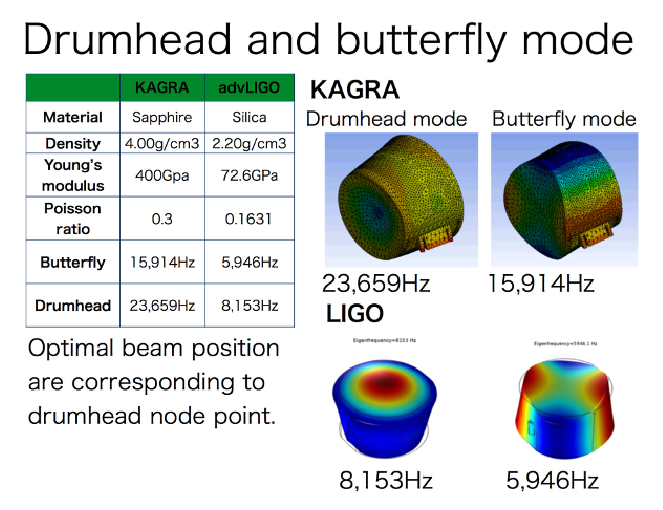
\includegraphics[width=14cm]{Figures/elmodes.eps}
\caption{Summary of drumhead and butterfly modes on KAGRA test mass 
compared with LIGO test mass.~\cite{Daveloza}} 
\label{fig:elmodes} 
\end{center}
\end{figure}

\begin{figure}
\begin{center}
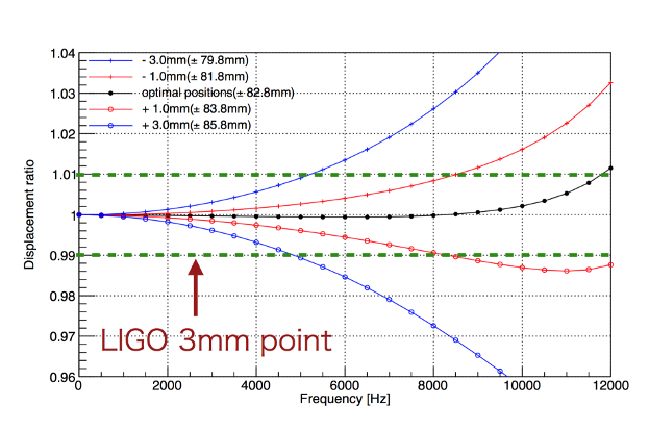
\includegraphics[width=14cm]{Figures/edeform.eps}
\caption{The ratio between the total sensed motion and rigid body motion 
as a function of frequency for optimally positoned baams and 
$\pm$1 mm and $\pm$3 mm offsets.} 
\label{fig:edeform} 
\end{center}
\end{figure}

%\section{Elastic deformation}
%\section{Summary}
